\documentclass[preview,convert={density=600,outext=.png}]{standalone}
%\documentclass[preview]{standalone}

\usepackage[utf8]{inputenc}				% Кодировка utf8

\usepackage{tikz}
\usetikzlibrary{calc,patterns,backgrounds}


\newcommand{\block}[3]{
	\node[draw, #3, rectangle, fill = #3, minimum width = #1, minimum height = #2] 
}
\newcommand{\blockp}[3]{
	\node[draw, rectangle, pattern = #3, minimum width = #1, minimum height = #2] 
}
\begin{document}
	
	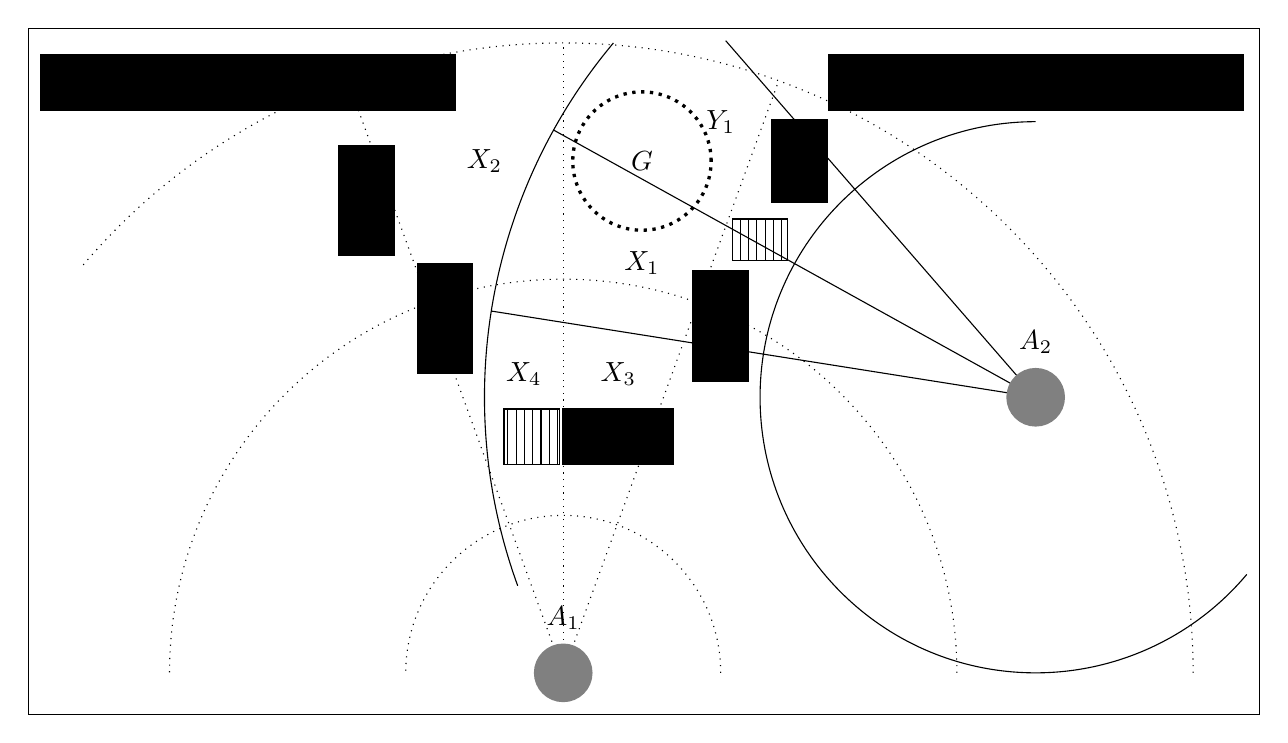
\begin{tikzpicture}[framed]

		\block{150}{20}{black} at (0,0) {};
		\block{150}{20}{black} at (10,0) {};
		
		\block{20}{40}{black} at (1.5,-1.5) {};
		\block{20}{40}{black} at (2.5,-3) {};
		
		\block{40}{20}{black} at (4.7,-4.5) {};
		\blockp{20}{20}{vertical lines} at (3.6,-4.5) {};
		
		\block{20}{40}{black} at (6,-3.1) {};
		\block{20}{30}{black} at (7,-1) {};
		\blockp{20}{15}{vertical lines} at (6.5,-2) {};
		
		\node[draw, circle, dotted, very thick, minimum width = 50, text = black] (goal) at (5, -1) {$G$};

		\draw[dotted] (4,-7.5) ++(0:2) arc (0:180:2);
		\draw[dotted] (4,-7.5) ++(0:5) arc (0:180:5);
		\draw[dotted] (4,-7.5) ++(0:8) arc (0:140:8);
		\draw[dotted] (4,-7.5) -- ++(90:8);
		\draw[dotted] (4,-7.5) -- ++(70:8);
		\draw[dotted] (4,-7.5) -- ++(110:8);

		\draw (10,-4) ++(90:3.5) arc (90:320:3.5);
		\draw (10,-4) ++(140:7) arc (140:200:7);
		\draw (10,-4) -- ++(151:7);
		\draw (10,-4) -- ++(131:6);
		\draw (10,-4) -- ++(171:7);
				
		\node[draw, gray, fill = gray, circle, very thick, minimum width = 20] (obj_1) at (4, -7.5) {};
		\node at (4, -6.8) {$A_1$};
		\node[draw, gray, fill = gray, circle, very thick, minimum width = 20] (obj_2) at (10, -4) {};
		\node at (10, -3.3) {$A_2$};
		

		\node at (5, -2.3) {$X_1$};
		\node at (3, -1) {$X_2$};
		\node at (4.7, -3.7) {$X_3$};
		\node at (3.5, -3.7) {$X_4$};
		\node at (6, -0.5) {$Y_1$};
	\end{tikzpicture}
\end{document}